\documentclass[9pt,twocolumn,twoside]{osajnl}


%\usepackage{csquotes}
\usepackage{tikz}
%\usepackage{graphicx}


\journal{josaa} % Choose journal (ao, josaa, josab, ol)

\setboolean{shortarticle}{false} % true = letter, false = research article


\title{On the using of the medium with variable optical axes as a curved space-time for light }

\author[1]{S. A. Mousavi}
\author[2*]{R. Roknizadeh}
\author[3,4]{SH. Dehdashti}
\author[5]{S. Sahebdivan}

\affil[1]{Department of Physics, Faculty of Science, University of Isfahan, Hezar Jerib, Isfahan, 81746-73441, Iran}
\affil[2]{ Department of Physics, Quantum Optics Group, Faculty of Science, University of Isfahan, Hezar Jerib, 81746-73441 Isfahan, Iran}
\affil[3]{State Key Laboratory of Modern Optical Instrumentations, Zhejiang University, Hangzhou 310027, China}
\affil[4]{The Electromagnetic Academy at Zhejiang University, Zhejiang University, Hangzhou 310027, China}
\affil[5]{Quantum Optics, Quantum Nanophysics and Quantum Information, Faculty of Physics, University of Vienna, Boltzmanngasse 5, 1090 Wien}
\affil[*]{Corresponding author: r.roknizadeh@gmail.com}

\dates{Compiled \today}

\ociscodes{(160.1190)  Anisotropic optical materials,(160.3918) Metamaterials, (260.2110)   Electromagnetic optics }

\doi{\url{http://dx.doi.org/10.1364/ao.XX.XXXXXX}}

\begin{abstract}


An optical impedance-matched medium with the gradient refractive index can resemble a geometrical analogy with an arbitrary curved space-time \cite{leonhardt2006general}. 
 In this paper, we show that a non-impedance-matched medium with a varying optical axis can also resemble the features of a metric for light.
The medium with a varying optical axis is an engineered stratified slab of material that the orientation of the optical axis in each layer would slightly differ from the other layers, while, the magnitude of refractive index remains constant. 
Instead of the change in the refractive index, the inhomogeneity of such a medium is induced by the local anisotropy.  Therefore, the propagation of light depends on the local optical axis.
We study the conditions that make the analogy between curved space-time and a medium with a varying optical axis. 
Extension of the transformation optics to the media with optical axis profile might ease some fabrication cumbersome of gradient refractive index materials for particular frequencies. 

\end{abstract}



\setboolean{displaycopyright}{true}

\begin{document}
\maketitle
\thispagestyle{fancy}
\ifthenelse{\boolean{shortarticle}}{\abscontent}{}

\section{Introduction}





 %-----------------------------------------------------------------------------------------------------------
\begin{figure}[top]
     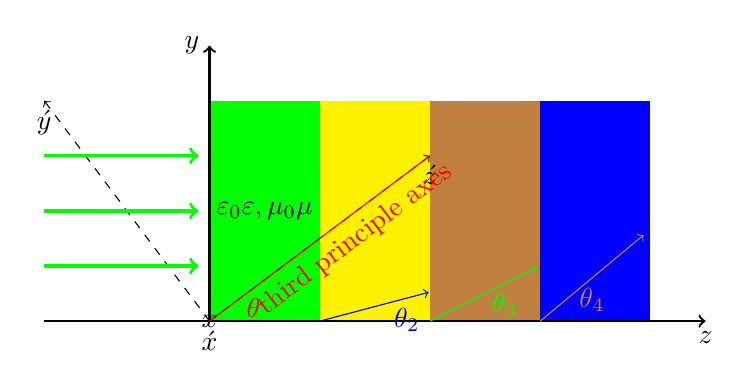
\begin{tikzpicture}[xscale=0.7, yscale=0.7]
                \fill[fill=green] (2,0) rectangle (4,4)node [pos=0.5]{$\varepsilon_0 \boldsymbol \varepsilon, \mu_0 \boldsymbol\mu $};
       \fill[fill=yellow] (4,0) rectangle (6,4);
           \fill[fill=brown] (6,0) rectangle (8,4);
            \fill[fill=blue!] (8,0) rectangle (10,4);
    %----------------------------------------------------------------------
            \draw [->,thick] (2,0) node{$x$} -- (2,5.0) node[left]{$y$} ;
        \draw [->,thick] (-1,0) -- (11,0) node [below]{$z$};
        \draw [-> ,dashed] (2,0)node [below]{$\acute{x}$} -- (6,3)  node [below]{$\acute{z}$};
     \draw [-> ,dashed] (2,0) -- (-1,4) node [below]{$ \acute{y}$};
    %----------------------------------------------------------------------
          \draw [red] (2,0) -- (6,3) node [pos=0.2, below]{$\theta$} node [pos=.6,below, rotate=37]{third principle axes} ;
           \draw [->,blue] (0:4) -- (5:6)node [pos=0.8, below]{$\theta_2$};
           \draw [->,green] (0:6) -- (7:8)node [pos=0.7, below]{$\theta_3$};
            \draw [->,brown] (0:8) -- (9:10)node [pos=0.5, below]{$\theta_4$};
        %---------------------------------------------------------------------------------
                    \draw [-> , green,very thick] (-1,1)  -- (1.8,1)  ;
        \draw [->,green,very thick] (-1,2)  -- (1.8,2) ;
            \draw [->,green,very thick] (-1,3)  -- (1.8,3)  ;       
    \end{tikzpicture}
    \caption{Schematic of an anisotropic slab with $\boldsymbol{\varepsilon}$ and $\boldsymbol{\mu}$ as a tensor, light incidents from left and incident plane is $y-z$ plane; two principle axes of media  $z^{\prime}$ and $y^{\prime}$ do not lay on the $z$ and $y$ coordinate.}\label{figure1}
\end{figure}
%---------------------------------------------------------------------------------------------


Transformation optics works based on the diffeomorphic map between a virtual space and the physical space. 
For technical simplicity, in most of the applications, physical space is constructed from an isotropic medium with a refractive index profile varies in position, while the optical axis remains fixed.
 This simplification restricts the underlying diffeomorphic map to the family of quasi-conformal maps. 
However, inspired by optical axes grating in liquid crystals \cite{Sarkissian, NERSISYAN}, one can show the diffeomorphic map between the virtual space and physical space might extend to the family of the area-preserving maps if one sequentially manipulates the direction of optical axes instead of gradually changing the amplitude of refractive index \cite{liang2012transformation}. 


In theory, an array of homogeneous anisotropic thin layers, which in each layer the direction of the principal axes is controllable, can form an inhomogeneous medium with optical axes profile.  
The inhomogeneity is induced by the local anisotropy and gradual change in the direction of the optical axes over space. The global inhomogeneity is responsible for curving the light trajectories. 

 This kind of medium can be realized, for example, by applying the external field or internally charged particles on the designed arrays of liquid crystals \cite{sluijter2010ray} or by other techniques that combines the arrays of homogeneous anisotropic layers together. Such materials show the capacity for being used in transformation optics designs when impedance-matched materials are costly. 
Unlike the most of the artificial metamaterials that are constructed from two kinds of meta-atom, the medium with variable optical axis can be fabricated from one kind of homogeneous anisotropic material \cite{liang2012transformation}.

From the practical perspective, unlike the impedance-matched media, anisotropic materials are accessible in nature, and even much cheaper to design artificially. Crystals are the best-known materials that perform electrical anisotropy based on their particular crystal structure and the symmetry of their space-group. Many plastics also are anisotropic, because their molecules are 'frozen' in a stretched conformation when the plastic is molded or extruded \cite{PEN}. 

 
In this research, considering a medium with the variable optical axis, we construct the optical metric in the plane of in propagation, for the extraordinary ray. Therefore, a medium with the variable optical axis can be considered as a curved space-time for extraordinary light rays. 
 
 In the final part of the paper, we study the anisotropic, impedance-matched medium. We show in details, instead of demanding the impedance-matched condition, for some applications, it is enough to restrict the concern only to the electrical response of the material and utilize the optical properties of an anisotropic birefringent medium. 
 
 
The paper organized as follows: 
In section \ref{method}, we briefly summarize the process of this research.
In section \ref{li}, we explain in details a technique, called eigenvalue wave equation method, to solve the Maxwell equations in the anisotropic medium. 
In section \ref{general-normal}, we apply the method to study the behavior of light in a normal incident on the single anisotropic slab.

In section \ref{m.v}, we derive the light trajectory for two examples where the array of the non-magnetic slabs forms a variable optical axes media. 

Further, we construct the optical metric for such media and discuss over the resulting curvature in the optical plane for light trajectories.

In the final section, as we mentioned, we studied the use of the birefringent medium in transformation optics.
Finally, in conclusion, some results and remarks are summarized. 

\section{ Method}\label{method}

The aim of this paper is to derive the effective optical metric for a stratified medium in which the anisotropy and homogeneity are only local. The medium as a whole is inhomogeneous.
We consider the medium consist of many thin slabs. Each slab assumes to be anisotropic and homogeneous. We are deriving the solutions of the wave equation in any single anisotropic layer with an arbitrary direction of the principle axes. Having the wave solutions for each slab, we can calculate the ray direction and consequently, achieve the ray trajectory in the system. 
According to the Fermat principle, light in a medium follows the geodesics. By studying the properties of the light geodesics in the medium, we might be able to associate a geometry to the medium. Particularly, it is possible to study the curvature of the effective metric.

\section{Light in anisotropic media}\label{li}

In mathematical term, the electric permittivity and magnetic permeability of anisotropic materials are described by a tensorial quantity. For most of the anisotropic media, there are two different refractive indexes associated with two normal modes. One of these refractive indexes, called extraordinary, depends on the orientation of the principle axes \cite{saleh1991fundamentals, born1999principles, yariv1984optical}, therefore, it is convenient to start studying the propagation of light in an anisotropic slab.

\subsection{Maxwell equations in  anisotropic media}\label{Maxwell's equations in the homogeneous anisotropic media}

 Maxwell's equations in an inhomogeneous anisotropic source-free materials, $\rho=0, \quad \mathbf{J}=0 $,  are given by \cite{jackson1962classical}:

\begin{gather}
\nabla\cdot \mathbf{D} =0,\quad \nabla\cdot \mathbf{B} =0, \nonumber \\
\nabla\times\mathbf{E}=-\dfrac{\partial\mathbf{B}}{\partial t}, \quad \nabla\times\mathbf{H} =\dfrac{\partial\mathbf{D}}{\partial t}.\label{m.h}
\end{gather}

While the constitutive relations are hold as:

 \begin{equation} 
 \mathbf {D}=\varepsilon_0 \boldsymbol \varepsilon \mathbf{E},  \qquad
  \mathbf{B}=\mu_0 \boldsymbol\mu \mathbf{H},
  \end{equation}
where $\boldsymbol{\varepsilon}$ and $\boldsymbol{\mu}$  are respectively the electric permittivity and  the magnetic permeability tensors for an arbitrary optical axis. 

 Explicitly assuming electric and magnetic anisotropy, wave equation can be written as
 
\begin{equation}
\mathbf{\nabla}\times{\boldsymbol{\mu^{-1}}(\mathbf{\nabla}\times\mathbf{E})}=-\mu_{0}\dfrac{\partial^{2}}{{\partial{t}}^{2}}\mathbf{D}.
\label{eq3}
\end{equation}

In a homogeneous anisotropic medium, the plane waves, $ \mathbf{E}\propto \exp\left[i\mathbf{k} \cdot  \mathbf{r}- i\omega t \right]$, is usually assumed as the general solution of the Maxwell wave equation \cite{hao2008electromagnetic}. Using this assumption, Eq. (\ref{eq3}) becomes:
   
   %------------------------------------------------------------------------------------------------------------
   \begin{equation}\label{w.eq}
    \mathbf{k}\times{\boldsymbol{\xi}(\mathbf{k}\times\mathbf{E})}=-k^{2}_{0}\boldsymbol{\varepsilon}\mathbf{E},
\end{equation}

where $\boldsymbol{\xi}=\boldsymbol{\mu}^{-1}$.
We rewrite the equation (\ref{w.eq}) in a matrix equation form, 
\[\mathbf{M}\mathbf{E}=-k_{0}^{2}\boldsymbol{\varepsilon}\mathbf{E}, \] 
in which  the matrix elements of $\mathbf{M}$ are obtained as

\begin{align}
M_{11}&=2\xi_{23}k_{z}k_{y}-(\xi_{33}k_{y}^{2}+\xi_{22}k_{z}^{2}), \nonumber\\
M_{12}&=\xi_{21}k_{z}^{2}-\xi_{23}k_{z}k_{x}-\xi_{31}k_{z}k_{y}+\xi_{33}k_{y}k_{x}, \nonumber\\
M_{13}&=\xi_{31}k_{y}^{2}-\xi_{23}k_{y}k_{x}-\xi_{21}k_{z}k_{y}+\xi_{22}k_{z}k_{x}, \nonumber\\
M_{22}&=2\xi_{13}k_{z}k_{x}-(\xi_{33}k_{x}^{2}+\xi_{11}k_{z}^{2}), \nonumber\\
M_{23}&=\xi_{32}k_{x}^{2}-\xi_{12}k_{z}k_{x}-\xi_{31}k_{y}k_{x}+\xi_{11}k_{y}k_{z},\nonumber\\
M_{33}&=2\xi_{21}k_{x}k_{y}-(\xi_{22}k_{x}^{2}+\xi_{11}k_{y}^{2}).
\end{align}


\subsection{Eigenvalue equation; method}

In an anisotropic material, the electric and magnetic components of the field are not necessarily perpendicular to the wave vector. The direction of the $ \mathbf{E} $ and $\mathbf{H} =$ fields can varies as light propagates through the medium.  However, the electric and magnetic induction are always perpendicular on the wave vector according to the relations through the relation: $\nabla\cdot \mathbf{D} =0 $ and $\nabla\cdot \mathbf{B} =0$.



So, it is useful to write the eigenvalue equation in term of $\mathbf{D}$  \cite{saleh1991fundamentals}. 
By defining the phase refractive index as a ratio between wave number in medium and in vacuum, $n=k/k_{0}$ and substituting $\boldsymbol{k}=nk_{0}\hat{U}$ in Eq. (\ref{w.eq}), we get eigenvalue equation, 

\begin{equation}\label{d.w.eq}
    \hat{U}\times{\boldsymbol{\xi}(\hat{U}\times\boldsymbol{\eta}\mathbf{D})}=-\frac{1}{n^{2}}\mathbf{D},
\end{equation}

where $\hat{U}=\mathbf{k}/k$ is a direction of the wave vector and $\boldsymbol{\eta}=\boldsymbol{\varepsilon}^{-1}$. Accordingly, we find  two directions for $\mathbf{D}$ correspond to  the wave vector.\\

 The Eq. (\ref{d.w.eq}) can be written in operator form,

\begin{equation}\label{m.f}
\mathbf{L}\mathbf{D}=-\frac{1}{n^{2}}\mathbf{D}.        
\end{equation}

In a general coordinate, matrix  $L$ might has a complicated form. Nevertheless, knowing that the light propagates in a plane, we can establish a fixed coordinate system such that the propagation plane coincides with one of the principal planes of the coordinate system. As  Fig. \ref{figure1} shows, we choose the $y-z$ as the propagation plane, so the $x$ component of  the wave vector vanishes.  Thus,  matrix $L$ simplifies to the following non-zero components:

\begin{align}
L_{1i} &= (\xi_{31}\eta_{3i}-\xi_{33}\eta_{1i})u^{2}_{2} +(-\xi_{22}\eta_{1i}+\xi_{21}\eta_{2i})u^{2}_{3}\nonumber\\
&\qquad +(2\xi_{23}\eta_{1i}-\xi_{31}\eta_{2i}-\xi_{21}\eta_{3i})u_{2}u_{3},\nonumber\\
L_{2i} &=(\xi_{12}\eta_{1i}-\xi_{11}\eta_{2i})u^{2}_{3}+(-\xi_{13}\eta_{1i}+\xi_{11}\eta_{3i})u_{2}u_{3}, \nonumber \\
L_{3i} &=(\xi_{13}\eta_{1i}-\xi_{11}\eta_{3i})u^{2}_{2}+(-\xi_{12}\eta_{1i}+\xi_{11}\eta_{2i})u_{2}u_{3},
 \end{align}
where $i=1,2,3$.

One can obtain electrical displacement $\mathbf{D}$  by solving  Eq. (\ref{m.f}) through the matrix algebra:


\begin{equation}\label{det}
    \det(\mathbf{L}+\frac{1}{n^{2}}\mathbf{I})=0,
\end{equation}

Having the components of  $\mathbf{D}$, other fields, and the Poynting vector can be calculated easily  \cite{jackson1962classical}

\begin{equation}\label{e.h}
\mathbf{E}=\frac{\boldsymbol\eta}{\varepsilon_{0}}\mathbf{D}, \hspace{.5cm}  \mathbf{B}=n\sqrt{\mu_{0}\varepsilon_{0}}  \hat{U}\times{\mathbf{E}}, \hspace{.5cm}\mathbf{H}=\frac{\boldsymbol\xi}{\mu_{0}}\mathbf{B},
\hspace{.5cm}\mathbf{S}=  \mathbf{E}\times \mathbf{H}.
\end{equation}

Finally, the direction of the field propagation for each mode is determined from the Poynting vector as: 

\begin{equation}\label{p.v}
\dfrac{\mathbf{\mathrm{d}{r}}}{\mathrm{d}{l}}=\dfrac{\mathbf{S}}{S}.
\end{equation}


\section{Normal incident of light on a piece of electromagnetic slab} \label{general-normal}

In this section, we investigate the behavior of the perpendicular incident light on a single anisotropic slab of material.
Our analyze is easily extendable to an arbitrary angle of incidence.
It is well known that in the normal incidence, the direction of the wave vector does not change.  We consider the $y-z$ plane as the propagation plane, while, the light comes parallel to the $z$ axis. Therefore:  

\begin{eqnarray}\label{pt}
|\mathbf{k}|=k_{z} \quad\rightarrow \quad {n}^{2}_{p}=n^{2}_{zz}.
\end{eqnarray} 

Further, we assume that two principal axes  $y^{\prime}$ and $z^{\prime}$ of the slab lay in the $y-z$ plane, Fig. \ref{figure1}.
In this case, the dielectric tensor can be obtained from following relation \cite{yeh1980optics},

 \begin{eqnarray}\label{t.t}
        \boldsymbol{\varepsilon}= \mathbf{A} \boldsymbol{\varepsilon^{\prime}}\mathbf{A}^{T},
\end{eqnarray}

where $ \boldsymbol{\varepsilon^{\prime}} = \mbox{diag} (\varepsilon_{1},\varepsilon_{2},\varepsilon_{3})$ are  principle permittivity tensors and $\mathbf{A}$  is the rotation matrix, which describes the rotation of the coordinate axes with respect to the crystal principle axes and $ \mathbf{A}^{T}$ is transpose of the rotation matrix $ \mathbf{A}$.

Suppose that two principal axes  $y^{\prime}$ and $z^{\prime}$ of the slab lay in this plane, Fig. \ref{figure1}, then the rotation matrix is given by
 
\begin{align}\label{r.m}
        \mathbf{A}=\mathbf{R}_{x}(\theta)=
        \begin{pmatrix}
            1&0&0 \\
            0&\cos{\theta} &\sin{\theta} \\
            0&-\sin{\theta} & \cos{\theta}
        \end{pmatrix},
\end{align}

where $\theta$ is a angle between $z$ and $z^{\prime}$.  From Eq. (\ref{t.t}),  we can obtain the rotated permittivity tensor,

\begin{align}\label{eps}
        \boldsymbol{\varepsilon}=
        \begin{pmatrix}
             \varepsilon_{1} &0 &0 \\
            0&\varepsilon_{2} \cos^{2}{\theta} + \varepsilon_{3}\sin^{2}{\theta}   &-(\varepsilon_{2}-\varepsilon_{3})\sin{\theta}\cos{\theta} \\
            0&-(\varepsilon_{2}-\varepsilon_{3})\sin{\theta}\cos{\theta} &\varepsilon_{2} \sin^{2}{\theta} + \varepsilon_{3}\cos^{2}{\theta}
        \end{pmatrix}.
\end{align}
and also the inverse permittivity tensor,

\begin{align}\label{eta}
        \boldsymbol{\eta}= \frac{1}{\varepsilon_{2} \varepsilon_{3}}
        \begin{pmatrix}
            \frac{\varepsilon_{2} \varepsilon_{3}}{\varepsilon_{1}}& 0  &0 \\
            0&\varepsilon_{2} \sin^{2}{\theta} + \varepsilon_{3}\cos^{2}{\theta}   & (\varepsilon_{2}-\varepsilon_{3})\sin{ \theta} \cos {\theta} \\
            0& (\varepsilon_{2}-\varepsilon_{3})\sin{\theta}\cos{\theta} &\varepsilon_{2} \cos^{2}{\theta} + \varepsilon_{3}\sin^{2}{\theta}
        \end{pmatrix}.
\end{align}

From Maxwell equations we have $\boldsymbol{\nabla}\cdot \mathbf{D}=0$, hence, for  the normal incident it reads as ${D}_{z}=0$.  
For other components of the $\mathbf{D}$ by replacing relation (\ref{eta}) in (\ref{d.w.eq}), we would have:

\begin{eqnarray}\label{z.d.eq}
        \begin{pmatrix}
            - \eta_{11} \xi_{22}  & \xi_{21}\eta_{22} \\
             \eta_{11} \xi_{12}& -\xi_{11}\eta_{22}
        \end{pmatrix}
        \begin{pmatrix}
            D_{x} \\ D_{y}
        \end{pmatrix}
        = -\frac{1}{n^{2}}
        \begin{pmatrix}
            D_{x} \\ D_{y}
        \end{pmatrix}.
        %\end{align}
\end{eqnarray}

By applying the condition (\ref{det}), the eigenvalues of the Eq. (\ref{z.d.eq}) are obtained from the following equation:

\begin{equation}\label{gn}
 \left( \dfrac{1}{n^2}- \eta_{11} \xi_{22}\right)\left(\dfrac{1}{n^2}-\xi_{11}\eta_{22}\right)-\xi_{21}^{2}\eta_{22}\eta_{11}=0
\end{equation}

This is a quadratic equation in terms of $1/n^2$ which has two eigenvalues;

\begin{equation}\label{general-n}
\dfrac{1}{n^2}=
\begin{cases}
\dfrac{\eta_{11} \xi_{22}+\xi_{11}\eta_{22}+ \sqrt{\left(\eta_{11} \xi_{22}-\xi_{11}\eta_{22}\right)^{2}+4\xi_{21}^{2}\eta_{11}\eta_{22}}}{2},\\
\dfrac{\eta_{11} \xi_{22}+\xi_{11}\eta_{22}- \sqrt{\left(\eta_{11} \xi_{22}-\xi_{11}\eta_{22}\right)^{2}+4\xi_{21}^{2}\eta_{11}\eta_{22}}}{2}.
\end{cases}
\end{equation}

Corresponding eigenvectors would determine the physical components of the field. 

In the next part, we investigate two special examples: a layer of a non-magnetic medium, with $\boldsymbol \mu=1$, and a slab of impedance-matched material, with $\boldsymbol \mu = \boldsymbol \varepsilon $. 

\subsection{Non-magnetic anisotropic medium}\label{electric anisotropic}

For the purely electric medium, the refractive indices (\ref{general-n}) are given by

\begin{eqnarray}
        &n_{o}^2=\varepsilon_{1} \label{n1},\\
        &n^{2}(\theta)=\dfrac{\varepsilon_{2}\varepsilon_{3}}{\varepsilon_{2}\sin^{2}{\theta}+\varepsilon_{3}\cos^{2}{\theta}} \label{n2}.
\end{eqnarray}    

Relation (\ref{n2}) shows the refractive index depends on principle values of the permittivity tensor, i.e., $\varepsilon_{2}$ and $\varepsilon_{3}$, and, $\theta$, the angle between the direction of the wave vector and third principle axis. Whereas the refractive index (\ref{n1})  depends only on $\varepsilon_{1}$.

For a specific angle of incident, in this example perpendicular incident, there are two modes associated with the above refractive indices profiles. 

For refractive index (\ref{n1}), we can obtain $\mathbf{D}$ by solving the eigenvalue equation (\ref{z.d.eq}):

\begin{align} \label{mod-n1}
        \mathbf{D}=D_{x}
         \begin{pmatrix}
            1 &0&0
         \end{pmatrix}^{T}.    
\end{align}

and for the refractive index (\ref{n2}) we have:

 \begin{eqnarray}\label{mod-n2}
  \mathbf{D}=D_{y}
\begin{pmatrix}
0&1&0
\end{pmatrix}^{T}.
 \end{eqnarray}
 
By applying the normalization condition, $\mathbf{E}\cdot \mathbf{E}=1$, we can determine the components $D_{x} $ and $D_{y} $. 
For the first normal mode (\ref{mod-n1}), electric and magnetic fields are written in the from (\ref{e.h}),

\begin{align}\label{field-n1}
\mathbf{E}=
         \begin{pmatrix}
             1\\0\\0
         \end{pmatrix},
        \qquad
         \mathbf{H}=\left(\frac{\varepsilon_{0}}{\mu_{0}}\right)^{\frac{1}{2}}(\varepsilon_{1})^{\frac{1}{2}}
         \begin{pmatrix}
            0\\1\\0
        \end{pmatrix}.
\end{align}

We can see that the normal mode is TE polarized light. The electrical component lies in the propagating plane $y-z$.
 For second normal mode (\ref{mod-n2}),  $\mathbf{E}$ and $\mathbf{H}$ are given by,

 \begin{eqnarray}
\mathbf{E}=\left(\varepsilon_{2}^{2} \sin^{2}{\theta} + \varepsilon_{3}^{2}\cos^{2}{\theta}\right)^{-\frac{1}{2}}
 \begin{pmatrix}
 0\\ \varepsilon_{2} \sin^{2}{\theta} + \varepsilon_{3}\cos^{2}{\theta}\\ (\varepsilon_{2}-\varepsilon_{3})\sin{\theta}\cos{\theta}
 \end{pmatrix},
\end{eqnarray}
\begin{eqnarray}
 \mathbf{H}=\left(\frac{\varepsilon_{0}}{\mu_{0}}\right)^{\frac{1}{2}}\left(\dfrac{\varepsilon_{2}\varepsilon_{3}\left(\varepsilon_{2} \sin^{2}{\theta} + \varepsilon_{3}\cos^{2}{\theta}\right)}{\varepsilon_{2}^{2}\sin^{2}{\theta}+\varepsilon_{3}^{2}\cos^{2}{\theta}}\right)^{\frac{1}{2}}
 \begin{pmatrix}
 -1\\0\\0
 \end{pmatrix}.
 \end{eqnarray}
It is worth mentioning that, while the TE polarized field is propagating along the electric flux density, modes with TM polarization do not. The Poynting vectors of TE and TM polarizations can derive as

 \begin{equation}\label{ordinary-s}
\mathbf{S}_{TE}= \left(\frac{\varepsilon_{0}}{\mu_{0}}\right)^{\frac{1}{2}}(\varepsilon_{1})^{\frac{1}{2}}
 \begin{pmatrix}
 0\\0\\1
 \end{pmatrix},
  \end{equation}
 
  \begin{align}\label{extra.s}
 \mathbf{S}_{TM}= \left(\frac{\varepsilon_{0}}{\mu_{0}}\right)^{\frac{1}{2}} &\dfrac{(\varepsilon_{2}\varepsilon_{3})^{\frac{1}{2}}({\varepsilon_{2}\sin^{2}{\theta}+\varepsilon_{3}\cos^{2}{\theta}})^{\frac{1}{2}}}{\varepsilon_{2}^{2} \sin^{2}{\theta} + \varepsilon_{3}^{2}\cos^{2}{\theta}}\nonumber \\
&\qquad \times\begin{pmatrix}
 0\\ -(\varepsilon_{2}-\varepsilon_{3})\sin{\theta}\cos{\theta}  \\  \varepsilon_{2} \sin^{2}{\theta} + \varepsilon_{3}\cos^{2}{\theta}
 \end{pmatrix}. 
 \end{align}
 
 The ray direction is given by the angle of the ray with respect to the z-axis, determined  by the relations (\ref{ordinary-s}), (\ref{extra.s}) and (\ref{p.v}).
 For the TE mode, we can write:

 \begin{equation}\label{ordinary-d}
\tan{\phi}=\dfrac{S_{y}}{S_{z}}=0, \qquad \dfrac{\mathbf{\mathrm{d}{r}}}{\mathrm{d}{l}}=
 \begin{pmatrix}
 0\\0\\1
 \end{pmatrix}.
\end{equation}

While for the TM mode, we achieve:

\begin{equation}\label{extra.d}\begin{split}
\tan\phi & =\dfrac{-(\varepsilon_{2}-\varepsilon_{3})\sin{\theta}\cos{\theta}}{\varepsilon_{2} \sin^{2}{\theta} + \varepsilon_{3}\cos^{2}{\theta}},\\
 \dfrac{\mathbf{\mathrm{d}{r}}}{\mathrm{d}{l}} & =\dfrac{1}{\sqrt{\varepsilon_{2}^{2} \sin^{2}{\theta} + \varepsilon_{3}^{2}\cos^{2}{\theta}}}
 \begin{pmatrix}
 0\\ -(\varepsilon_{2}-\varepsilon_{3})\sin{\theta}\cos{\theta}  \\  \varepsilon_{2} \sin^{2}{\theta} + \varepsilon_{3}\cos^{2}{\theta}
 \end{pmatrix}.
\end{split}\end{equation}

Since the wave vector is along the z-axis, $\phi$ is equivalent to the deviation angle of the light from the wave vector direction.
In the relation (\ref{extra.d}), the propagation direction of TM polarization is not identical with the wave vector. Therefore, it represents extraordinary ray, whereas the ray direction of TE polarization is along the wave vector and, therefore, it is the ordinary ray. 

 
\section{Medium with variable optical axes}\label{m.v}

In this section we investigate the effective space-time perceived by light rays in a medium that its principal axes orientation depends only on $z$ direction: $\theta=\theta(z)$;
As in the previous section, we consider the inhomogeneous medium as stratified layers of homogeneous, anisotropic slabs in the $z$ direction as in the  Fig. \ref{figure1}. The principle axis of each slab is varying in the $y-z$ plane. 

\subsection{Ray tracing}
We apply the ray-tracing method to trace the light geodesics in two example of planar media with variable optical axes:
First, a medium in which the orientation of optical axes varies with $z$ as $\theta=z$, and the second one where the dependency of the optical axis to z direction follows the relation: $\theta=\sqrt{z}$. Also, we assume that the principle values of permittivity are equal to  $\varepsilon_{2}=2.75$ and $\varepsilon_{3}=2.21$, which is associated to the calcite crystal principal permittivities \cite{yariv1984optical}. 
 
 According to the relation {\ref{extra.d}} we can trace the extraordinary light in layered anisotropic media using solving the following equation:
 \begin{eqnarray}
\mathrm{d}{y}=\dfrac{-(\varepsilon_{2}-\varepsilon_{3})\sin{\theta(z)}\cos{\theta(z)}}{\varepsilon_{2} \sin^{2}{\theta(z)} + \varepsilon_{3}\cos^{2}{\theta(z)}}\mathrm{d}{z}
\end{eqnarray}
 
   In Fig. \ref{curvedspace2}, the plotted trajectories of the family of extraordinary rays are shown. Left and right diagrams are corresponding to the $\theta=z$ and $\theta=\sqrt{z}$ respectively, which indicates the normal incidence of light. 

\begin{figure}[htbp]
\centering
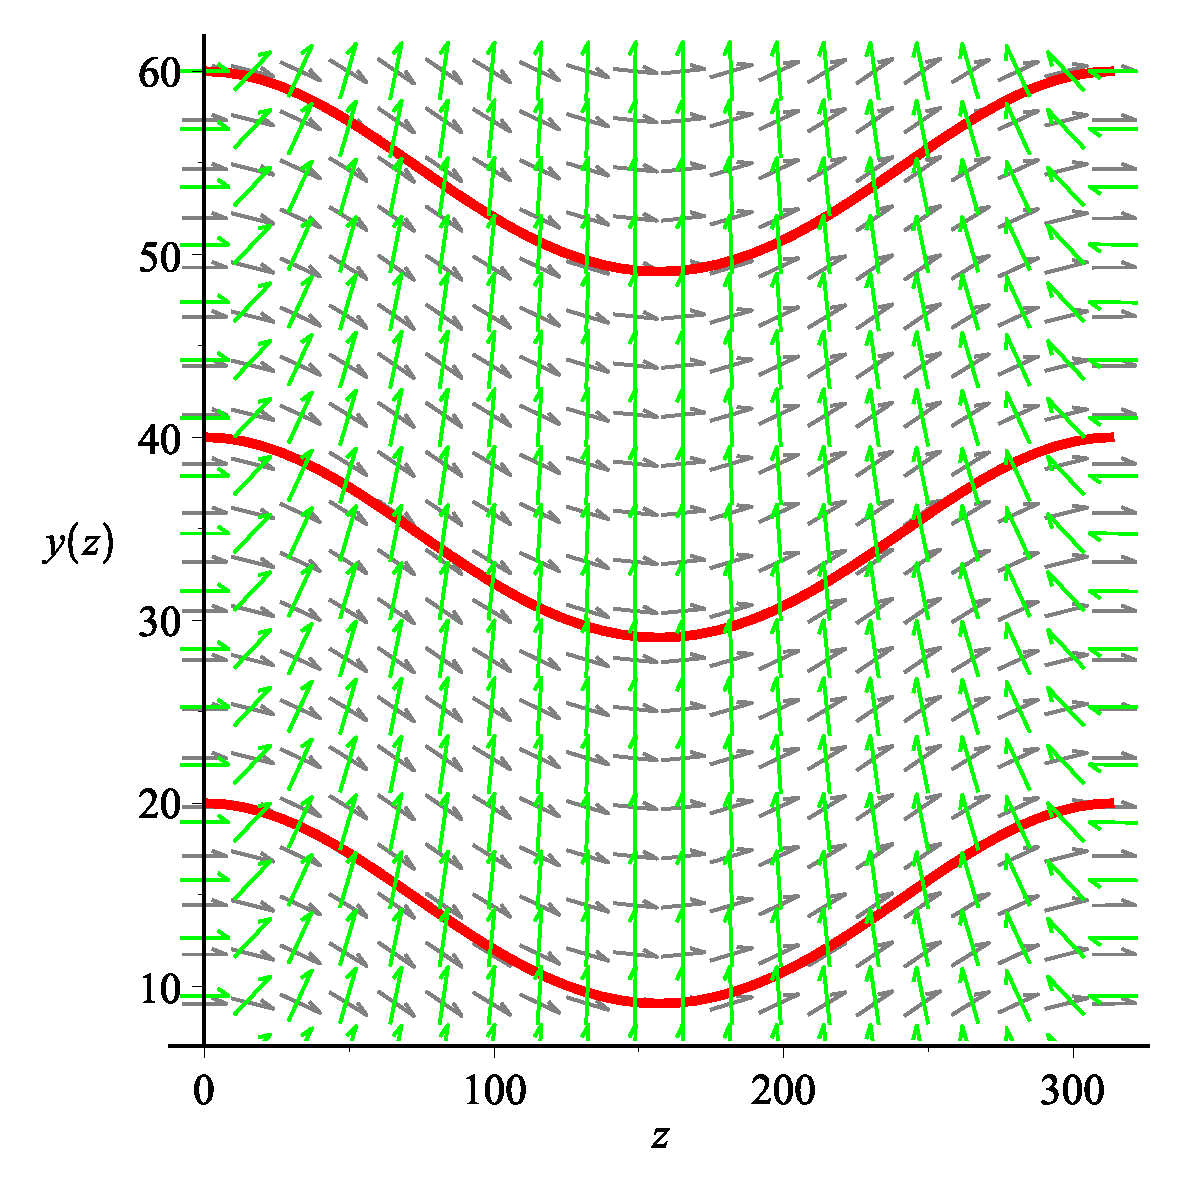
\includegraphics[scale=0.2]{Visualization4}
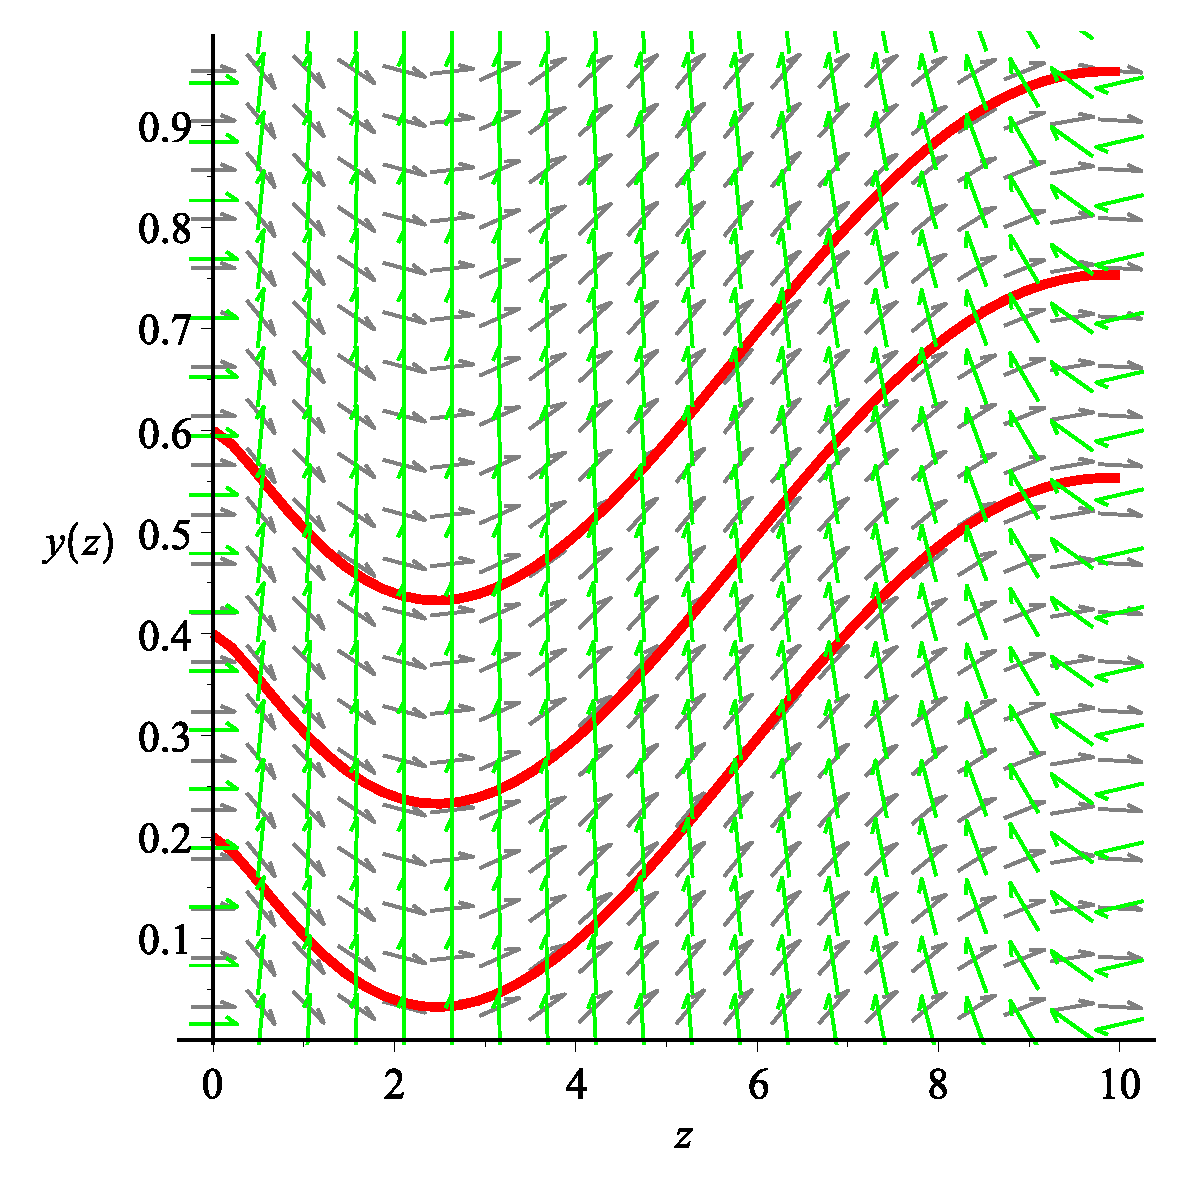
\includegraphics[scale=0.2]{Visualization3}
\caption{Ray tracing in anisotropic media with variable optical axes, $\theta=z$ (left) and $\theta=sqrt{z}$ (right), the  green arrows  indicate orientations of the third principle axis and the red lines  indicate ray trajectories  in the media.}
\label{curvedspace2}
\end{figure}

As we can see in the Fig.\ref{curvedspace2}, the light geodesics through these media are not straight lines and moreover, it seems that these surfaces are under tension. Therefore, we expect a non-zero Riemann tensor for the corresponding metric.  
 
\subsection{Metric}
 
we can construct the  metric of  this two dimensional distorted surface, Fig \ref{curvedspace2}, by choosing two bases of this space as:
\begin{eqnarray}\label{base}
e_{1}=c_{1}
\begin{pmatrix}
1\\0
\end{pmatrix}, \qquad
e_{2}=c_{2}
\begin{pmatrix}
0\\1
\end{pmatrix},
\end{eqnarray}

 where coefficients $c_{1}$ and $c_{2}$  are scalar functions which provides sufficient conditions for null geodesics  $\mathrm{d}s^{2}=0$. Using these bases (\ref{base}), the metric components \cite{leonhardt2012geometry} are  given by:
 
\begin{eqnarray}
g_{ij}=e_{i}\cdot e_{j}.
\end{eqnarray}

Therefore, we can write the space-time metric in the matrix form as,   
\begin{equation}
\mathbf{g}=
\begin{pmatrix}
-1&0&0\\
0&c_{1}&0\\
0&0&c_{2}
\end{pmatrix}
\end{equation}

or equivalently in the form of the Riemann line element as,
\begin{eqnarray}\label{gl}
\mathrm{d}s^{2}=-c^{2}dt^{2}+c_{1}^{2} dy^{2} +c_{2}^{2} dz^{2}
\end{eqnarray}
The null geodesics condition,$\mathrm{d}s^{2}=0$,  results,
\begin{eqnarray}
 c_{1}^{2} dy^{2} +c_{2}^{2} dz^{2}-c^{2}dt^{2}=0
\end{eqnarray}
We can assume $c_{1}=c_{2}$, so we achieve
\begin{eqnarray}\label{c1c2}
c_{1}^{2}=c_{2}^{2} =\dfrac{c^{2}dt^{2}}{dl^{2}}
\end{eqnarray}
where $dl^{2}=dy^{2}+dz^{2}$.

On the other hand, for the light fields, the surfaces of the equal phases define as the solutions of:

\begin{equation}\label{level}
\mathrm{d}{\varphi(r,t)}=0.
\end{equation}

This condition (\ref{level}) results in: 

\begin{equation}\label{phase1}
\mathbf{k}\cdot {\mathrm{d}\mathbf{r}}-\omega\mathrm{d}{t}=0.
\end{equation}
our equivalently
\begin{equation}
c dt=n\hat{U}\cdot {\mathrm{d}\mathbf{r}}
\end{equation}.

Equation (\ref{imp-d}) and (\ref{extra.d}) results in the following relation:


\begin{eqnarray}\label{cdt}
c dt=\dfrac{\varepsilon_{2} \sin^{2}{\theta} + \varepsilon_{3}\cos^{2}{\theta}}{\sqrt{\varepsilon_{2}^{2} \sin^{2}{\theta} + \varepsilon_{3}^{2}\cos^{2}{\theta}}}dl
\end{eqnarray}
Substituting (\ref{cdt}) in relation (\ref{c1c2}) the coefficient $c_{1}$ and $c_{2}$ are easily determined,
\begin{eqnarray}
c_{1}^{2}=c_{2}^{2}=n\dfrac{\left(\varepsilon_{2} \sin^{2}{\theta} +\varepsilon_{3}\cos^{2}{\theta}\right)^{2}}{\varepsilon_{2}^{2} \sin^{2}{\theta} + \varepsilon_{3}^{2}\cos^{2}{\theta}}
\end{eqnarray}
Substituting the $c_{1}$ and $c_{2}$ in the relation (\ref{gl}) the line element of the propgation plane can be written as
\begin{eqnarray}\label{general-metric}
\mathrm{d}s^{2}=-c^{2}dt^{2}+ n\dfrac{\left(\varepsilon_{2} \sin^{2}{\theta} + \varepsilon_{3}\cos^{2}{\theta}\right)^{2}}{\varepsilon_{2}^{2} \sin^{2}{\theta} + \varepsilon_{3}^{2}\cos^{2}{\theta}}dl^{2}
\end{eqnarray}

Using the refractive index  achieved in the previous section, (\ref{n2}), we can construct the following optical metric for the extraordinary ray:

\begin{eqnarray}\label{el-metric}
ds^{2}=-c^{2}dt^{2} + \dfrac{\varepsilon_{2}\varepsilon_{3}\left({\varepsilon_{2} \sin^{2}{\theta} + \varepsilon_{3}\cos^{2}{\theta}}\right)}{\left({\varepsilon_{2}^{2} \sin^{2}{\theta} + \varepsilon_{3}^{2}\cos^{2}{\theta}}\right)} {(dy^{2}+dz^{2})}.
\end{eqnarray}

Careful attention to the relation (\ref{el-metric}) implies the conformally flat nature of the two-dimensional space, which associates with the spatial part of the metric with the following refractive index:

\begin{equation}
n_{ray}(\theta)=\dfrac{\varepsilon_{2}\varepsilon_{3}\left({\varepsilon_{2} \sin^{2}{\theta} + \varepsilon_{3}\cos^{2}{\theta}}\right)}{\left({\varepsilon_{2}^{2} \sin^{2}{\theta} + \varepsilon_{3}^{2}\cos^{2}{\theta}}\right)}
\end{equation}

Where index $n_{ray}$ is the effective refractive indexes perceived by light rays. According to the varying profile of the optical axes, this refractive index  can take the values between 
$\sqrt{\varepsilon_{2}}$ and $\sqrt{\varepsilon_{3}}$. 


Although this range is small in natural anisotropic crystals, can varies greater in the designed anisotropic metamaterials.



\subsection{Curvature} 

The line element (\ref{el-metric}) indicate that the propagation plane is a conformally flat space with (possibly) non-zero curvature. 
We can investigate the curvature by using the differential geometry relations.


 Riemann curvature tensor is given by \cite{leonhardt2012geometry}
\begin{equation}\label{Riemann}
R^{i}_{jkl}\equiv \Gamma^{i}_{jl,k}-\Gamma^{i}_{jk,l}+\Gamma^{i}_{mk}\Gamma^{m}_{jl}-\Gamma^{i}_{ml}\Gamma^{m}_{jk}
\end{equation}

where $\Gamma^{i}_{jk}$ is the Christoffel symbol and the comma notation "$,$" refers to partial differentiation.  The Christoffel symbol can be expressed in terms of the metric components as,

\begin{equation}\label{cr}
\Gamma^{i}_{jk}=\dfrac{1}{2} g^{il}(g_{lj,k}+g_{lk,j}-g_{jk,l})
\end{equation}

For the metric (\ref{el-metric}}), which is a two-dimensional conformally flat space, $g_{ij}=n^{2}\delta_{ij}$,  we can obtain Christoffel symbol  from relation,

\begin{equation}\label{cr1}
\Gamma^{i}_{ij}=\dfrac{1}{2n^{2}}n^{2}_{,j}.
\end{equation}
Using the relation, (\ref{cr1}), Riemann curvature tensor, (\ref{Riemann}) is achieved as:
\begin{equation}

\begin{split}
&R_{11}=R_{22}=\\
&\dfrac{1}{2n^{4}} \lbrace (\dfrac{\partial}{\partial z}n^{2})^{2} +(\dfrac{\partial}{\partial y}n^{2})^{2}\rbrace -\dfrac{1}{2n^{2}}\lbrace(\dfrac{\partial}{\partial z}\dfrac{\partial}{\partial z}n^{2})+(\dfrac{\partial}{\partial y}\dfrac{\partial}{\partial y}n^{2})\rbrace
\end{split}
\end{equation}

We calculated this tensor for the above mentioned example of the medium with variable axes , $\theta=z$. Consequently, we find that the  curvature is non-zero,

 \begin{equation}
R_{ii}\neq 0.
\end{equation}

The media with $\theta=f(z)$ have a non-zero Riemann curvature tensor and appear as a curved space for the extraordinary light. Therefore, it is possible to use the variable optical axes media for realizing the curved space-time in the laboratory. 

\section{impedance-matched anisotropic medium}\label{impedance-matched}
In this section using the relations achieved in section \ref{general-normal}, we investigate the behaviour of the normal incident light on the impedance-matched anisotropic slab, $ \mu_{ij} =\varepsilon_{ij} $ and then compare its results with the case of the electric medium.
For the impedance-match anisotropic medium,  $ \mu_{ij} =\varepsilon_{ij} $,  two refractive indexes (\ref{general-n}) reduce to the one relation:

\begin{align}\label{impedance-match index}
n_{imp}^{2}(\theta)=\dfrac{\varepsilon_{1}\varepsilon_{2}\varepsilon_{3}}{\varepsilon_{2}\sin^{2}{\theta}+\varepsilon_{3}\cos^{2}{\theta}}.
\end{align}
Therefore, alike the birefringent media, for the impedance-matched medium we have one eigenvalue, i.e. the impedance matched media do not birefringence. For more investigation we compared this medium with the electric medium result achieved in previous subsection. By comparing the refractive indices (\ref{impedance-match index}) with (\ref{n2}), we find that,

\begin{equation}\label{comper-n}
n_{imp}(\theta)=\sqrt{\varepsilon_{1}}n_{el}(\theta),
\end{equation}
where index el (imp) stands for  electric (impedance-matched). ${\varepsilon_{1}}$ govern the electrical responses of the ordinary mode in birefringent medium,
\begin{equation}\label{comper-n1}
n_{imp}^{2}(\theta)=n_{o}^{2}n_{el}^{2}(\theta).
\end{equation}

 Also, we investigate the behavior of the birefringent medium normal mode, TE and TM polarization, in the impedance-matched medium.
 
Following the Eq. (\ref{e.h}),  for the TM mode, the electric and magnetic field are given by,

 \begin{align}
  \mathbf{E}=\left(\varepsilon_{2}^{2} \sin^{2}{\theta} + \varepsilon_{3}^{2}\cos^{2}{\theta}\right)^{-\frac{1}{2}}
 \begin{pmatrix}
 0\\
  \varepsilon_{2} \sin^{2}\theta + \varepsilon_{3}\cos^{2}\theta\\
 (\varepsilon_{2}-\varepsilon_{3})\sin\theta\cos\theta
 \end{pmatrix},
\end{align}
\begin{align}
  \mathbf{H}=\left(\frac{\varepsilon_{0}}{\mu_{0}}\right)^{\frac{1}{2}}\dfrac{(\varepsilon_{1}\varepsilon_{2}\varepsilon_{3})^{\frac{1}{2}}({\varepsilon_{2}\sin^{2}{\theta}+\varepsilon_{3}\cos^{2}{\theta}})^{\frac{1}{2}}}{(\varepsilon_{2}^{2} \sin^{2}{\theta} + \varepsilon_{3}^{2}\cos^{2}{\theta})^{\frac{1}{2}}}
 \begin{pmatrix}
 -1\\0\\0
 \end{pmatrix}.
 \end{align}
While for the TE polarization the electric and magnetic field became,

\begin{equation}\label{e-te-im}
\mathbf{E}=
 \begin{pmatrix}
 1&0&0
 \end{pmatrix}^{T},
\end{equation}
\begin{align}\label{h-te-im}
\begin{split}
  \mathbf{H}= \left(\frac{\varepsilon_{0}}{\mu_{0}}\right)^{\frac{1}{2}}&\dfrac{(\varepsilon_{1}\varepsilon_{2}\varepsilon_{3})^{\frac{1}{2}}}{({\varepsilon_{2}\sin^{2}{\theta}+\varepsilon_{3}\cos^{2}{\theta}})^{\frac{1}{2}}}\dfrac{1}{\varepsilon_{2}\varepsilon_{3}}
  \\ & \qquad\times
  \begin{pmatrix}
  0\\
 \varepsilon_{2} \sin^{2}\theta + \varepsilon_{3}\cos^{2}\theta\\
 (\varepsilon_{2}-\varepsilon_{3})\sin\theta\cos\theta
 \end{pmatrix}.
\end{split}
\end{align}

Expressions (\ref{e-te-im}) and (\ref{h-te-im}) show that for the TE mode, the electric field $\mathbf{E}$ and displacement field $\mathbf{D}$, are in the same direction. While, the magnetic field $\mathbf{H}$ is not along the induction $\mathbf{B}$, whereas for the  TM mode it is the opposite.


From relation (\ref{p.v}), we obtain the Poynting vector for the TM and TE modes in impedance-matched medium

\begin{align}\label{s}
\begin{split}
  \mathbf{S}_{TM}=\left(\frac{\varepsilon_{0}}{\mu_{0}}\right)^{\frac{1}{2}}&\dfrac{(\varepsilon_{1}\varepsilon_{2}\varepsilon_{3})^{\frac{1}{2}}({\varepsilon_{2}\sin^{2}{\theta}+\varepsilon_{3}\cos^{2}{\theta}})^{\frac{1}{2}}}{\varepsilon_{2}^{2} \sin^{2}{\theta} + \varepsilon_{3}^{2}\cos^{2}{\theta}}
\\& \qquad\times
 \begin{pmatrix}
 0\\ -(\varepsilon_{2}-\varepsilon_{3})\sin{\theta}\cos{\theta}  \\  \varepsilon_{2} \sin^{2}{\theta} + \varepsilon_{3}\cos^{2}{\theta}
 \end{pmatrix},
 \end{split}
 \end{align}
\begin{align}\label{p.v 2}
\begin{split}
\mathbf{S}_{TE}=\left(\frac{\varepsilon_{0}}{\mu_{0}}\right)^{\frac{1}{2}}&\dfrac{(\varepsilon_{1}\varepsilon_{2}\varepsilon_{3})^{\frac{1}{2}}}{({\varepsilon_{2}\sin^{2}{\theta}+\varepsilon_{3}\cos^{2}{\theta}})^{\frac{1}{2}}}\dfrac{1}{\varepsilon_{2}\varepsilon_{3}}
\\ &\qquad\times
\begin{pmatrix}
 0 \\ -(\varepsilon_{2}-\varepsilon_{3})\sin\theta\cos\theta \\   \varepsilon_{2} \sin^{2}\theta + \varepsilon_{3}\cos^{2}\theta
 \end{pmatrix}.
 \end{split}
\end{align}

It is clear that both TE and TM modes have the same Poynting vector. Consequently, light in impedance-matched media is not divided into ordinary and extraordinary rays as it is expected.
The angle between ray and z-axis can be written as,

\begin{align}\label{tanp}
\tan{\phi}_{(TE)}=\tan{\phi}_{(TM)}=\frac{-(\varepsilon_{2}-\varepsilon_{3})\sin{\theta}\cos{\theta}}{\varepsilon_{2} \sin^{2}{\theta} + \varepsilon_{3}\cos^{2}{\theta}}.
\end{align}
Also, we can write the ray direction in the impedance-matched slab as 
\begin{equation}\label{imp-d}
\dfrac{\mathbf{\mathrm{d}{r}}}{\mathrm{d}{l}}=\dfrac{1}{\sqrt{\varepsilon_{2}^{2} \sin^{2}{\theta} + \varepsilon_{3}^{2}\cos^{2}{\theta}}}
 \begin{pmatrix}
 0\\ -(\varepsilon_{2}-\varepsilon_{3})\sin{\theta}\cos{\theta}  \\  \varepsilon_{2} \sin^{2}{\theta} + \varepsilon_{3}\cos^{2}{\theta}
 \end{pmatrix}.
\end{equation}
Relation (\ref{imp-d})  shows important fact about the impedance-matched media; The ray direction in the impedance-matched medium do not necessarily a long the wave vector. In these media although the birefringent effect do not occur, but the ray direction in this medium is the extraordinary ray.  Comparison between (\ref{extra.d}) and (\ref{imp-d}) shows  

\begin{equation}\label{compare-direction}
\left(\dfrac{\mathbf{\mathrm{d}{r}}}{\mathrm{d}{l}}\right)_{el}^{TM}= \left(\dfrac{\mathbf{\mathrm{d}{r}}}{\mathrm{d}{l}}\right)_{imp},
\end{equation}

The direction of the rays in impedance-matched media is the same as the direction extraordinary rays in the non-magnetic anisotropic media.

\subsection{Ray tracing and metric}

Fig. \ref{curvedspace2} (drew according to the relation (\ref{compare-direction}) ) shows the ray trajectory in the impedance-matched, inhomogeneous medium with  $\theta=z$ and $\theta=\sqrt{z}$.

While, the corresponding effective metric, of the plane of propagation, can be achieved from the relation (\ref{general-metric}),

\begin{eqnarray}
\mathrm{d}s^{2}=-c^{2}dt^{2}+ n\dfrac{\left(\varepsilon_{2} \sin^{2}{\theta} + \varepsilon_{3}\cos^{2}{\theta}\right)^{2}}{\varepsilon_{2}^{2} \sin^{2}{\theta} + \varepsilon_{3}^{2}\cos^{2}{\theta}}dl^{2}
\end{eqnarray}



 The impedance matched-media appears as following metric for the light ray:

\begin{equation}\label{metric-im}
ds^{2}=- c^{2}dt^{2} + \dfrac{\varepsilon_{1}\varepsilon_{2}\varepsilon_{3}\left({\varepsilon_{2} \sin^{2}{\theta} + \varepsilon_{3}\cos^{2}}\right)}{\left({\varepsilon_{2}^{2} \sin^{2}{\theta} + \varepsilon_{3}^{2}\cos^{2}}\right)} {(dy^{2}+dz^{2})}.
\end{equation}

On the other hand, using the methods of transformation optics \cite{leonhardt2012geometry}, the spatial metric for an impedance-matched medium achieved from 

\begin{equation}
\mathbf{g}=(\det{ \boldsymbol{\varepsilon}})\boldsymbol{\varepsilon}^{-1}.
\end{equation}

The spatial metric in our example, Fig. \ref{figure1}, take the following form: 

\begin{align}\label{t-metric}
&\mathbf{g}_{imp}(y-z)= \nonumber\\
&\begin{pmatrix}
\varepsilon_{1}(\varepsilon_{2} \sin^{2}{\theta} +\varepsilon_{3}\cos^{2}{\theta})& \varepsilon_{1}(\varepsilon_{2}-\varepsilon_{3})\sin{\theta} \cos{\theta}\\
\varepsilon_{1}(\varepsilon_{2}-\varepsilon_{3})\sin{\theta} \cos{\theta}&\varepsilon_{1}(\varepsilon_{2} \cos^2{\theta} +\varepsilon_{3}\sin^{2}{\theta})
\end{pmatrix}.
\end{align}

At first glance, the metric (\ref{t-metric}) looks different from the our constructed metric (\ref{metric-im}), but by using the following relation:  

\begin{equation}\label{dz}
\begin{split}
\varepsilon_{2} \varepsilon_{3}&=(\varepsilon_{2} \cos^2{\theta} +\varepsilon_{3}\sin^{2}{\theta})(\varepsilon_{2} \sin^{2}{\theta} +\varepsilon_{3}\cos^{2}{\theta})  \\
&   \qquad  -\left[ (\varepsilon_{2}-\varepsilon_{3})\sin{\theta} \cos{\theta}\right]^{2},
\end{split}
\end{equation}
 we show that the two metrics (\ref{metric-im}) and (\ref{t-metric}) are equivalent.
 This equivalence can be considered as a verification of our method. 
 
\subsection{comparing between the metrics }

In this part, we discuss how transformation optics would apply to the non-impedance-matched media. 
Remember from \ref{general-normal}, the direction of the extraordinary ray in each point (\ref{extra.d}) in non-magnetic medium is coincide with direction of the rays in corresponding impedance-matched  version (\ref{imp-d}).  The relation (\ref{comper-n}) shows the two refractive indexes only differ up to a factor, i.e. $\varepsilon_{1}$. 

Therefore, we expect a similarity in their optical path length if $\varepsilon_{1}=$ constant.

 Mathematically, we consider the metrics (\ref{metric-im}) and (\ref{el-metric}); Temporal parts of these metrics are equal but their spatial part is not the same. Using null geodesics condition, we can write the following metric, (\ref{metric-T-1}) as a conformal equivalent  of the metric (\ref{el-metric}), 
\begin{equation}\label{metric-T-1}
ds_{el}^{2}=- \varepsilon_{1}c^{2}dt^{2}+\dfrac{\varepsilon_{1}\varepsilon_{2}\varepsilon_{3}\left({\varepsilon_{2} \sin^{2}{\theta} + \varepsilon_{3}\cos^{2}}\right)}{\left({\varepsilon_{2}^{2} \sin^{2}{\theta} + \varepsilon_{3}^{2}\cos^{2}}\right)}dl^{2}.
\end{equation}
Now, the spatial part of this metric, (\ref{metric-T-1}), is the same with the spatial part of the metric (\ref{metric-im}),
\begin{align}\label{metric-imp-c}
ds_{imp}^{2}=- c^{2}dt^{2}+\dfrac{\varepsilon_{1}\varepsilon_{2}\varepsilon_{3}\left({\varepsilon_{2} \sin^{2}{\theta} + \varepsilon_{3}\cos^{2}}\right)}{\left({\varepsilon_{2}^{2} \sin^{2}{\theta} + \varepsilon_{3}^{2}\cos^{2}}\right)}dl^{2}.
\end{align}

 Therefore, if $\varepsilon_1=constant$,  two metrics are conformally equivalent. A non-magnetic anisotropic medium, which is  not impedance-matched, appears for the TM polarized light (extraordinary light), like the impedance-matched medium for the non-polarized light. It seems that we can write this equivalence between these metrics as the following general relation:
 \begin{align}
\mathbf{g}_{el}(2+1)=
\begin{pmatrix}
-\varepsilon_{1}&0&\\
0&\mathbf{g}_{imp}(y-z)
\end{pmatrix}.
\end{align}

 As the result, for suitably polarized light, we can use non-magnetic medium instead of the impedance-match one to make the geometry exact. 
 More elaborated theory of using non-impedance-matched media as an alternative to impedance-matched media discuss in the further publications.
 
\section{Conclusion}\label{conclusion}

In this paper, we studied a particular kind of optical medium. The medium with the variable optical axis which is an engineered inhomogeneous material: The stratified medium forms from the array of homogeneous thin layers with controllable optical axes.  
We show that this uncommon form of inhomogeneity would also result in the emergence of effective geometry in the medium. Our finding results in a new method to manipulate the electromagnetic waves. More elaborated theory of transformation optics with variable optical axes profile would appear shortly in the further publications.

In the last part of the paper, we have studied the propagation of normal incident light in two kinds of medium with the similar anisotropy in their refractive index profile:  One fulfills the impedance-matched condition and the another posses only the electrical anisotropy. 
For the non-magnetic medium, we have the birefringence, namely, the split of ordinary and the extraordinary modes.  For the extraordinary mode, we have shown the direction of rays depend on the principle values of the permittivity tensor and the orientation of the principal axes.
While, in the impedance-matched media, the light rays do not split; there is a single direction of propagation for each angle of incidence.  
We conclude that the direction of propagation in the impedance-matched medium coincides with the direction of the extraordinary rays in the non-magnetic medium when both posses the same anisotropy in their refractive index.





\section*{Acknowledgment}
S.A.M, R.R wish to thank the office of graduate studies at the University of Isfahan for their support.

\bibliography{mybib}

\end{document}